\Chapter{NumPy hatékonyságának vizsgálata}

\section{Vektor és mátrix
műveletek}\label{vektor-uxe9s-muxe1trix-mux171veletek}

\subsection{Vektor műveletek:}\label{vektor-mux171veletek}

    Pythonban a \emph{NumPy} csomag használatával könnyedén definiálhatunk
vektorokat és mátrixokat. Ahhoz, hogy használhassuk előtte telepíteni
kell majd be kell a pip csomagkezelővel, majd az alábbi módon lehet
importálni:

\begin{python}
import numpy as np
\end{python}

    Ez a szintaktikája pythonban egy csomag inportálásának az \texttt{as}
operátor után aliast adhatunk a csomagnak, így megkönyítve a
használatát. Alias megadása nem kötelező.

    Ebben. esetben \texttt{np}-vel tudunk hivatkozni a \emph{NumPy}
csomagra. A csomagból az \texttt{array} metódus segítségével hozhatunk
létre vektorokat.

\begin{python}

\end{python}


    Üres vektort a következőképpen készíthetünk: az \texttt{empty}
metódusban meg kell adni szögletes zárójelek között egy dimenziót
(például: \texttt{{[}1,\ 3{]}} ez azt jelenti 1 sort és 3 oszlopot
szeretnénk), és esetlegesen megadhatunk neki egy adattípust, hogy milyen
adatokkal szeretnénk feltölteni.

    Itt főleg valmilyen numerikus adattípusra kell gondolni, hisz ezekkel
tudjuk elvégezni a vektor és mátrix műveleteket. Haszálhatjuk a python
beépített típusait mint az \texttt{int} vagy a \texttt{float}, de
használhatjuk a \emph{NumPy}-ban definiált kiegészített változatokat
amivel megadhatjuk azt például, hogy hány bájton tároljuk az adott
számot. Esetlegesen megadhatunk stringet és bool típust is ha szükség
van rá.

\begin{python}

\end{python}

\begin{python}

\end{python}

\begin{python}

\end{python}

\begin{python}

\end{python}

\begin{python}

\end{python}

\begin{python}

\end{python}

\begin{python}

\end{python}


    Ahogy láthatjuk, nem 0-ákkal tölti fel a vektort hanem valamilyen
memória szeméttel. Ennek az oka nagyon egyszerű: így gyorsabb, mint ha
nullázná az elemeket, de ha 0-ákkal szeretnénk feltölteni használhatjuk
a \texttt{zeros} metódust mely hasonló képpen működik mint az
\texttt{empty}:

\begin{python}

\end{python}

\begin{python}

\end{python}

    1-esekkel is feltölthetjük ehez a \texttt{ones}metódust használhatjuk:

\begin{python}

\end{python}

\begin{python}

\end{python}

    Létrehozhatunk egy bizonyos értékkel vagy pszeudóvéletlen (random)
számokkal feltöltött vektorokat is :

\begin{python}

\end{python}

\begin{verbatim}
[[0.22541693 0.47521003 0.90312494]]
[['aaa' 'aaa' 'aaa']]
\end{verbatim}

    A fent létrehozott \texttt{v1}, \texttt{v2}, \texttt{v3} vektorainkal
már egyszerűen elvégezhetőek a vektor műveletek, mint például az
összeadás:

\begin{python}

\end{python}

    vagy a kivonás:

\begin{python}

\end{python}

    vektoriális szorzás:

\begin{python}

\end{python}

    és a skaláris szorzás:

\begin{python}

\end{python}

    vagy számmal a való szorzás:

\begin{python}

\end{python}

    ha egyszerűen a összeszorozzuk a két vektort akkor a megfelelő hely lévő
tagokat szorozaz össze:

\begin{python}

\end{python}

    Transzponálhatjuk is a vektorainkat a \texttt{transpose} metódussal bár
vektorok esetén itt nem látványos:

\begin{python}

\end{python}

    Komolyabb műveletek mint a vektor normák kiszámítása is egyszerű. Vegyük
először az 1-es normát:

\begin{python}

\end{python}

    Itt használtuk a numpy \texttt{linalg} csomagját melyben előre
definiálva vannak a különbőző lineáris algebrához tartozó műveletek,
módszerek. Most nézzük a 2-es és a végtelen normát:

\begin{python}

\end{python}

    Mind itt a vektorműveleteknél és majd a mátrix műveleteknél sem árt
figyelni, hogy megfelelő dimenziójú vektorokat, mátrixokat adjunk meg a
műveletekhez, különben könnyen hibát vagy helytelen eredményt kaphatunk.

    \subsection{Mátrixok:}\label{muxe1trixok}

    A Mátrixok létrehozása is többféleképpen történhet hasonlóképpen mint a
vektoroknál. Legegyszerűbb módszer az ha megadjuk mi, hogy milyen
mátrixot szeretnénk vagy képezhetjük vektorokból is, estleg a fent
megismert \texttt{empty,\ zeros,\ ones,\ random.rand,\ full}
metódusoknak megadjuk a nekünk megfelelő dimenziókat.

   \begin{python}

\end{python}

\begin{verbatim}
m1
 [[1 2 4]
 [2 3 4]]
m2
 [[1 2 8]
 [2 3 9]]
m3
 [[1 2]
 [2 3]
 [4 5]]
m4
 [[1 2]
 [3 4]]
\end{verbatim}

\begin{python}

\end{python}

\begin{python}

\end{python}

    A \texttt{reshape}-nél vigyázni kell, hogy pontosan akkora elemszámú
mátrixot adjunk meg mint amekkora a mostani mátrixunké, különben hibát
kapunk.

\begin{python}

\end{python}

    Az \texttt{eye} metódu segítségével képezhetünk \(n*n\)-es
egységmátrixot, paraméterként a dimenziót kell megadnunk.

\begin{python}

\end{python}

\begin{verbatim}
[[1. 0. 0.]
 [0. 1. 0.]
 [0. 0. 1.]]
\end{verbatim}

    A vektorokhoz hasonlóan adhatjuk meg a mátrix műveleteket is, mint az
összeadást, kivonást, szorzást, normát:

\begin{python}

\end{python}

\begin{python}

\end{python}

\begin{python}

\end{python}

    Forbenius norma:

\begin{python}

\end{python}

    Végtelen norma:

\begin{python}

\end{python}

    1-es norma:

\begin{python}

\end{python}

    2-es norma

\begin{python}

\end{python}

    A transzponálás is hasonlóan működik:

\begin{python}

\end{python}

\begin{python}

\end{python}

    Egy négyzetes mátrix determinánsát is egyszerűen és gyorsan
kiszámíthatjuk a \texttt{linalg.det} metódussal:

\begin{python}

\end{python}

\begin{python}

\end{python}

\begin{python}

\end{python}

    Egy elemet az \texttt{item} metódussal tudunk kiválasztani, de figyelni
kell, mert az indexelés 0-tól kezdődik:

\begin{python}

\end{python}

    A mátrixokat feldarabolhatjuk a \texttt{hsplit} és \texttt{vsplit}
metúdusok segítségével. A \texttt{hsplit} oszlopok mentén, míg a
\texttt{vsplit} sorok mentén vágja el a megadott mátrixot.

\begin{python}

\end{python}

\begin{python}

\end{python}

\begin{python}

\end{python}

    Használhatjuk vágásra az \texttt{{[}{]}} operátorokat is, ha csak egy
paramétert adunk meg neki akkor az adott indexű sort kapjuk vissza, ha
használjuk a \texttt{:} operátort akkor megadhatunk neki intervallumot
is, hogy hanyadik sornál kezdje, megadhatunk neki lépésközt is illetve
részeket is kivághatunk egy adott mátrixból

\begin{python}

\end{python}

    Ha adunk meg neki lépésközt, akkor az az utolsó paraméter. Pl: az egész
mátrix minden párátlan számú sorának és oszlopának a közös elemei.

\begin{python}

\end{python}

    \subsection{Mátrix felbontások}\label{muxe1trix-felbontuxe1sok}

    \subsubsection{LU felbontás}\label{lu-felbontuxe1s}

    Mátrixok LU felbontásásval kinyerhetjük a felső- ,alsóháromszög
mátrixot. Pythonban erre használható a\texttt{Scipy.linalg.lu} metódus
ami a \texttt{SciPy} tudományos csomagban találhatunk meg ami egy
kiegészítése tulajdon képpen a \texttt{NumPy}-nak. Először telepíteni és
importálni kell ezt a csomagot és utána használatba lehet venni. Az
\texttt{lu} metódus végeredményként visszaadja az alsó-, felső-, és a
permutáció mátrixokat.

\begin{python}

\end{python}

    \begin{verbatim}
[[ 1.20000000e+01  1.30000000e+01  1.40000000e+01  1.50000000e+01]
 [ 0.00000000e+00  1.00000000e+00  2.00000000e+00  3.00000000e+00]
 [ 0.00000000e+00  0.00000000e+00 -4.44089210e-16 -9.99200722e-16]
 [ 0.00000000e+00  0.00000000e+00  0.00000000e+00  5.55111512e-16]]
    \end{verbatim}

    \subsubsection{Cholesky felbontás}\label{cholesky-felbontuxe1s}

    A Cholesky féle felbontásra is találunk beépített metódust a
\texttt{Numpy}-ban \texttt{cholesky} néven a \texttt{linalg} csomagban.
Cholesky felbontásnál vigyázni kell hogy a mátrixunk szimmetrikus legyen
és pozitív definit ellenben hibaüzenetet kapunk. Ugyan ez megtalálható a
\texttt{SciPy} csomagban is és a különbség az, hogy a \texttt{NumPy}-ban
lévő metódus az alsó-, addig a \texttt{SciPy}-ban lévő a felsőháromszög
mátrixot számolja.

\begin{python}

\end{python}

\begin{python}

\end{python}

    A fenti kód hibát eredményezett, mert a megadott mátrix nem volt pozitív
definit. A következő cellában már pozitív definit mátrixra van példa.

    \begin{python}

\end{python}

    De akár megírhatjuk a saját felbontó függvéníünket is:

   \begin{python}

\end{python}

    Mint ahogy láthajuk a metódus megadja egy közelítő megoldását a cholesky
felbontásnak.

\section{Lineáris
egyenletrendszerek}\label{lineuxe1ris-egyenletrendszerek}

    \subsection{Általánosan a lineáris
egyenletredszerekről}\label{uxe1ltaluxe1nosan-a-lineuxe1ris-egyenletredszerekrux151l}

    A lineáris egyenletrendszer egy többismeretlenes egyenletrendszer
melyben az ismeretlenek az első hatványon vannak.

    Egy \(n\) egyenlet és \(m\) változó esetén az egyenletrendszer általános
alakja a következő:

    \[
x_{1,1} + x_{1,2} + \dots + x_{1,m} = b_{1}\\
x_{2,1} + x_{2,2} + \dots + x_{2,m} = b_{2}\\
\vdots\\
x_{i,1} + x_{i,2} + \dots + x_{i,m} = b_{i}\\
\vdots\\
x_{n,1} + x_{n,2} + \dots + x_{n,m} = b_{n}\\
\]

    Aztmondjuk hogy az egyenlet rendszer alulhatárolt, hogyha \(n<m\) és
túlhatárolt, hogyha \(n>m\). Négyzetesnek nevezzük ha \(m=n\). Az
egyenletrendszer geometriai tartalmát az alábbi módon írhatjuk le:

    Az \(R^n\) euklideszi tér \(d\in R^n\) normálvektorú és \(x_0 \in R^n\)
ponton átmenő hipersíkját az

\[ (x - x_0)^Td=0\]

egyenletet kielégítő \(x \in R^n\) pontok határozzák meg.

    Az \(Ax=b\) egyenletrendszert felírhatjuk ilyen formában is:

    \[ 
a_{1}^Tx= b_1\\
a_{2}^Tx= b_2\\
\vdots\\
a_{n}^Tx= b_n\\
\]

    ahol \(a_{i}^T={a_{i1}, \dots a_{im}}\).

    Innen láthatjuk, hogy az egynletrendszer megoldása az \(m\) hipőersík
közös része, ennek megfelelően 3 megoldás lehetséges: 1. lehetőség:
nincs megolás 2. lehetőség: pontosan egy megoldása van 3. lehetőség:
végtelen sok megoldás van

    \paragraph{\texorpdfstring{\emph{Egynetrendszer
konzisztenciája:}}{Egynetrendszer konzisztenciája:}}\label{egynetrendszer-konzisztenciuxe1ja}

    \emph{Ha az \(Ax=b\) egyenletrendszernek legalább egy megoldása létezik
konzisztensnek nevezzük. Ha nem létezik egyetlen megoldása sem, akkor az
egyenletrendszer inkonzisztens.}

    \subsection{Lineáris egyenletrendszerek megoldása Pythonban, NumPy
csomag
segítségével}\label{lineuxe1ris-egyenletrendszerek-megolduxe1sa-pythonban-numpy-csomag-seguxedtsuxe9guxe9vel}

    Egy egyenletrendszert megoldani pythonban nem nehéz. A \texttt{NumPy}
tartalmazza a \texttt{solve} metódust mellyel könnyedén megoldható
egy-egy lineáris egyenletrendszer. A \texttt{solve} a \texttt{NumPy}
linalg csomagjában található, paramáterként várja az \(A\)
együtthatómátrixot és a \(b\) megoldásvektort. Nézzük is meg:

Vegyünk először egy egyszerű egyenletrendszert, mint ez: \[
    2x_1 + 9x_2 + 8x_3 + 7x_4= 7\\
    3x_1 - 2x_2 + 6x_3 + 4x_4= 4\\
    5x_1 + 8x_2 + 4x_3 + 7x_4= 2\\
    6x_1 + 9x_2 + 10x_3 + 2x_4= 6
\]

ezután importáljuk a numpy csomagot

\begin{python}

\end{python}

    Miután ezzel megvagyunk hozzuk létre az együttható métrixunkat és a
megoldás vektorunkat:

\begin{python}

\end{python}

    Majd használjuk a \texttt{solve} metódust

\begin{python}

\end{python}

\begin{python}

\end{python}

    A solve az Intel Math Kernel Library-ben megtalálható LAPACK gesv rutint
használja.

    A futás időt is kiírattam itt, hogy később össze lehessen vetni a
beépített és az általam implementált algoritmust. Az \texttt{allclose}
és\texttt{dot} metódusok segítségével pedig le is ellenőrízhetjük az
eredményt.

\begin{python}

\end{python}

\begin{python}

\end{python}
        
    Ilyen egyszerű az egész, de ha nem szeretnénk az előre megírt metódust
alkalmazni akkor definiálhatunk saját magunk is nekünk tetsző megoldó
metódust is. Például implementálhatjuk a Gauss módszert is. Ám mielőtt
ezt megnéznénk vessünk egy pillantást a ciklusokra pythonban csak, hogy
érthető legyen a kód.

    \paragraph{Rang}\label{rang}

    Egy lineáris egyenletrendszer csak akkor megoldható ha az A matrixunk
rangja megyegyezik a {[}A,b{]} mátrix rangjával ilyenkor az
egyenletrendszerünknek pontosan egy megoldása van. Ezt pythonban a
következő képpen tudjuk ellenőrizni:

\begin{python}

\end{python}

   \begin{python}

\end{python}

    Amint látjuk a két rang megegyezik ezáltal megoldható az itt látható
egyenlet rendszer.

    \paragraph{Ciklusok pythonban:}\label{ciklusok-pythonban}

    Pythonban is megtalálható a \texttt{for} és a \texttt{while} ciklus. A
\texttt{for} végig iterál egy iterálható objektumon ami pythonban lehet
egy tömb, string vagy az általunk kreált iterálható struktúra.

\begin{python}

\end{python}

    Ha klasszikus értelemben szeretnénk használni (tehát egy ciklus változót
léptetni egy kezdő értéktől egy végértékig) használnunk kell a
\texttt{range} metódust mely generál egy tömböt a megadott paraméterek
alapján. Három paramétere van, az első a kezdő érték, a második a
végérték és a harmadik a lépésköz. A \texttt{range} esetében figyelni
kell, mert a végéertékig generálja a számokat ezért a végérték nem
szerepel az általa vissza adott tömbben.

   \begin{python}

\end{python}

    A \texttt{while} működése nem tér el a többi általános célú programozási
nyelvben megszokottól. Amíg a megadott feltételünk igaz addig maradunk a
ciklusban.

\begin{python}

\end{python}

\begin{python}

\end{python}

    Nézzük még meg az \texttt{if} elágazást is mely megvizsgál egy logikai
kifejezést és annak értéke szerint ágaztatja el a programot.

  \begin{python}

\end{python}

    És akkor lássuk a Gauss módszer implementációját:

    \paragraph{Gauss módszer pythonban:}\label{gauss-muxf3dszer-pythonban}

   \begin{python}

\end{python}

    Láthatjuk futás időben elég közel van a numpyban lévő megoldáshoz. De
nem kapunk olyan pontos eredményt.

    Tegyünk most kis kitérőt a számítási munkára ezt valahogyan mérni kell,
hogy megtudjuk adni egyes algoritmusoknak a műveletigényét és ennek a
mértékegysége a flop. Egy régi flop az a számítási munk ami az
\(s=s+x*y\) művelet (egy összeadés és egy szorzás) elvégzéséhez kell, 1
új flopp pedig az a számítási munka mely egyetlen művelet (mindegy az
hogy additív vagy multiplikatív) elvégzéséhez szükséges. Az új flop
bevezetését az indokolta, hogy a mai számítógépeken a multiplikatív és
az additív műveletek elvégzéséhez szükséges idő azonosnak tekinthető.

    A gauss módszer $\dfrac{n^3}{3} + O(n^2)$ addítív és ugyanennyi
multiplikatív műveletet igényel, így a művelet igénye:\(\dfrac {n^3}{3}+
O(n^2) \) régi flop és \(\dfrac {2n^3}{3}+ O(n^2) \) új flop.

    \paragraph{Főelem kiválasztás}\label{fux151elem-kivuxe1lasztuxe1s}

    A fenti algoritmus csak olyan mátrixokat képes megoldani amikben egyik
együttható sem nulla. Hogy képes legyen rá ki kell egészíteni főelem
kiválasztással. A főelem kiválasztás azt jelenti, hogy a sorokat úgy
cseréljük fel, hogy az aktuális pivot elemünk ne legyen nulla. A
főelemkiválasztás lehet részleges vagy teljes. Részleges főelem
kiválasztásnál a \(k\)-adik lépésben megkeressük a \(k\)-adik oszlop
elemei közül a maximális abszolút értékű \(a_{ik}\) együtthatót és ez az
\(j\)-edik sorban van akkor megcseréljük a \(j\)-edik és a \(k\)-adik
sort. Ezzel fogunk majd találkozni a gauss-Jordan módszer
implementációjánál. A teljes főelem kiválasztás során pedig a \(k\)-adik
lépésben megkeressük a mátrixban szereplő értékek közül a maximális
abszolút értékűt és ha ez a \(a_{ij}\) akkor a \(k\)-adik sort
felcseréljük az \(i\)-edikkel és a \(k\)-adik oszlopot is felcseréljük a
\(j\)-edikkel.

    \paragraph{Gauss-Jordan módszer
pythonban}\label{gauss-jordan-muxf3dszer-pythonban}

    Egy másik lehetséges módszer az egyenletrendszerek megoldására a
Gauss-Jordan módszerezt leimplementálhatjuk mi magunk is, de én most egy
másik csomagot a SymPy-t fogom segítségül hívni. Első lépésnek vegyük az
\(A\) mátrixunkat és a \(b\) vektorunkat, majd használjuk az A mátrixra
definiált \texttt{gauss\_jordan\_solve} mmetódust melynek paraméterként
a \(b\) vektort adjuk meg. A metódus két visszatérési értéke a megoldás
és a mátrix.

\begin{python}

\end{python}

    Fontos, hogy a Matrixot nem kompatibilis az np.arrayel, így az értékeket
nekünk kell áthelyezni.

    Van egy 4. módszer is a lineáris egyenlet rendszer megoldására a
\texttt{scipy} csomagban, ami az lu faktorizáción alapul. A metódus neve
pedig \texttt{lu\_solve} és az alábbi módon lehet használni:

\begin{python}

\end{python}

    Most lássunk egy összesítő táblázatot a 3 módszerről:

\begin{python}

\end{python}


 \section{Interpolációk}\label{interpoluxe1ciuxf3k}

    \subsection{Általánosan az
interpolációkról}\label{uxe1ltaluxe1nosan-az-interpoluxe1ciuxf3kruxf3l}

    Az interpolációk alapfeladata az, hogy egy \(f(x)\) függvény felvett
értékeit különböző \(x_1, x_2 x_3 \dots x_n\) pontokban ismerjük az
\([a,b](a=x_1, b=x_n)\) intervallumban és magát az \(f\) függvényt
szeretnénk közelíteni egy könnyen számolható \(h(x)\) függvénnyel,
amelyre fenáll, hogy \(f(x_i)=h(x_i)\). Az \({x_i}_{i=1}^n\) pontokat
interpolációs alappontoknak, a feltételt interpolációs feltételnek
nevezzük. Az interpolációs feltétel teljesülése esetén azt reméljük,
hogy az interpoláló \(h(x)\) függvény jól közelíti az \(f(x)\) függvényt
az \([x_i,x_i+1]\) intervallumokban. Itt a Lagrange, Hermit és Spline
interpolációkról fogok elsősorban írni.

    Legegyszerűbben interpolációt ai \texttt{interp1d} metódussal tudunk
végre hajtani. ez a metódus nem kér csak \(x,y\) értékeket és a
interpoláció módját. A metódus a scipy.interpolate csomagban található
meg.

\begin{python}

\end{python}

    \begin{center}
%    \adjustimage{max size={0.9\linewidth}{0.9\paperheight}}{output_4_0.png}
    \end{center}
    { \hspace*{\fill} \\}
    
    Látható az \texttt{interp1d} egy függvénnyel tér vissza aminek csak meg
kell adnunk az \(x\) értékeinket és vissza adja az eredményt. Ezek
használhatóak a legkönnyebben pythonban. fontos, hogy miután elvégeztük
az interpolációt adott pontokra a függvénynek azonos intervallumon de
több alpontot tartalmazó tömböt adjunk át kirajzolásnál, hogy szépen és
pontosan rajzolja ki a közelítő függvénytés.

    Míg az \texttt{interp1d} \(y=f(x)\) típusú függvényeket interpolál addig
ennek a metódusnak a párja az \texttt{interp2d} már az \(z=f(x, y)\)
tipusú egyenleteket tudja közelíteni. használata az
\texttt{interp1d}-hez hasonló.

\begin{python}

\end{python}

    \begin{center}
%    \adjustimage{max size={0.9\linewidth}{0.9\paperheight}}{output_7_0.png}
    \end{center}
    { \hspace*{\fill} \\}
    
    Másik egyszerűen használható metódus a numpy csomagban található
\texttt{interp1d}. Az \texttt{interp1d} esetében meg kell adni az \(x\)
és \(y\) értékeinket illetve egy olyan intervallumot az \([a,b]\)
intervallumon ami több alpontot tartalmaz. A megadott alpontok számától
függ a pontosság tehát lehetőleg elég sokat adjunk meg. Az
\texttt{interp1d} szakaszokra ad meg lineáris interpolácót.

\begin{python}

\end{python}

    \begin{center}
    %\adjustimage{max size={0.9\linewidth}{0.9\paperheight}}{output_9_0.png}
    \end{center}
    { \hspace*{\fill} \\}
    
    \subsection{Lagrange interpoláció}\label{lagrange-interpoluxe1ciuxf3}

    Legyenek a \(\phi_i\) bázisfüggvények a következők
\(\phi_1=1, \phi_2=x, \dots , \phi_n=x^{n-1}\) és legyenek
\(x_1, x_2,\dots, x_n\) alpontjaink és \(y_i=f(x_i)\) az alpontokhoz
tartozó függvény értékek. Ekkor a feladatunk az, hogy határozzuk meg a
legfeljebb n-1-ed fokú \(p\) polinomot amelyre igaz, hogy
\(p(x_i)=y_i\). Ez tulajdonképpen az alapfeladat a lényegi rész az, hogy
ezt a \(p\) polinomot hogyan állítjuk elő. A Lagrange féle előállítás a
következőképpen néz ki:

    \[
l_i(x)=\prod_{k=1, k\neq i}^n\frac{x-x_k}{x_i-x_k}
\] Majd ezekhez az \(l_i\) értékeket megszorozzuk a \(y_i\) értékeket és
megkapjuk a \(p\) polinomot. \[
p(x)=\sum_{i=1}^n y_il_i(x)
\]

    Ezáltal meg kapjuk az \(f(x)\) függvényünk közelítését a \(p(x)\)
polinom által. (\(f(x) \approx p(x)\))

    Pythonban a scipy.interpolate csomag \texttt{lagrange} függvényével
tudunk a lagrange interpolációt számolni. Figyelni kall hogy egy poly
nevű változóba tér vissza.

\begin{python}

\end{python}

    \begin{center}
    %\adjustimage{max size={0.9\linewidth}{0.9\paperheight}}{output_15_0.png}
    \end{center}
    { \hspace*{\fill} \\}
    
    Látszik a pontosság itt is fögg a megadott alpontok számától. Bár a
lagrange interpolációnak létezik pythonos implementációja numerikusan
unstabil ezért ha mindenféleképpen ezt szeretnénk használni érdemesebb a
saját implementációnkat elkészíteni.

    \subsection{Spline interpoláció}\label{spline-interpoluxe1ciuxf3}

    Spline interpoláció esetén is megvannak az \(x_i\) pontjaink és \(y_i\)
függvényértékeink és ezek mellett keressük azt az \(S(x)\) függvényt
mely teljesíti az alábbi feltételeket: \[
S(x)= S_i(x)\quad x\in[x_i, x_{i+1}]\\
S(x_i)= y_i\quad (i=1, \dots, n)\\
S_i(x_{i+1})= S_{i+1}(x_{i+1})\quad (i=1, \dots, n-2)\\
\]

    Az első feltétel megfogalmazza,hogy szakaszokból áll a függvényünk, a
második megmondja, hogy valóban interpoláló függvény az \(S(x)\)
függvényünk és a harmadikkal a folytonosság van definiálva az \([a,b]\)
intervallumon.

    A spline meghatározásánál felírunk \(n\) darab \(k\)-ad fokú polinomot
ebből látszik, hogy az ismeretlenek száma \(n(k+1)\). Az első és a
harmadik feltételből következik az, hogy a feltételek száma
\((k+1)n-(k-1)\), ugyanis \(k-1\) db simasági feltétel a \(n-1\) belső
pontban ebből jön az, hogy \((n-1)(k-1)\) és \(2n\) interpolációs
feltétel. Összesen \((n-1)(k-1)+2n=(k+1)n-(k-1)\) és ebből látszik, hogy
hiányzik a spline egyértelműségéhez még \(k-1\) darab feltétel. Ezeket a
végpontokra szokták megadni.

    Vegyük először a lineáris spline interpolációt ebben az esetben a
\(k=1\) és a három feltétel egyértelműen meghatározza. Minden
\([x_k, x_{k+1}]\) intervallumon: \[
S_k(x_k)=a_kx_k+b_k=y_k \\
S_k(x_{k+1})=a_kx_{k+1}+b_k=y_{k+1}\\
\] Ebből a kétismeretlenes egyenletrendszerből meghtározható \(a_k\) és
\(b_k\).

    Beszélhetünk még kvadratikus splineokról is ebben az esetben \(k=2\) és
\(k-1 = 1\) feltétel hiányzik a spline egyértelmű felírásához. Ezt a
feltételt általában az intervallum elején vagy végén a derivált
megadásával szokás teljesíteni. Az így felvázolt esetben az egymás
melletti intervallumokra Hermite interpolációt alkalmazva meghatározható
a spline.

    Gyakorlatban azonban a harmadfokú spline interpolációt használjuk
túlnmyómó részt és csak harmadfokú splineról beszélünk, viszont ezek
további feltételek felírását követelik meg: \[
S_i'(x_{i+1})= S_{i+1}'(x_{i+1})\quad (i=1, \dots, n-2)\\
S_i''(x_{i+1})= S_{i+1}''(x_{i+1})\quad (i=1, \dots, n-2)\\
S''(x_{1})= A_n \quad \textrm{és} \quad S''(x_{n})=B_n
\]

    Pythonban használhatjuk a harmadfokú splinet is ehez elő kell készíteni
a scipy.interpolate csomagban megtalálható \texttt{splprep} metódussal
majd utána tudjuk használni a \texttt{splev} metódust ami a harmadfokó
splinet adja vissza.

    Először vegyünk egy függvényt és pár alpontot legyen most ez a sinus
függvény és próbáljuk ezt közelíteni spline-al.

\begin{python}

\end{python}

    \begin{center}
    %\adjustimage{max size={0.9\linewidth}{0.9\paperheight}}{output_26_0.png}
    \end{center}
    { \hspace*{\fill} \\}
    
    Látható hogy a harmadfokó spline jól közelíti a függvényünket hiszen
nagyjából lefedi és a megadott pontokban felveszi az értéket a megadott
értékeket.

    \subsection{Hermite interpoláció}\label{hermite-interpoluxe1ciuxf3}

    A harmadik interpoláció amit csak megemlítek az a Hermite interpoláció.
Hermite interpoláció esetén ugyan úgy megvannak az
\(x_0, x_1, \dots, x_n \in [a,b])\) pontjaink, mint eddig és vannak
mellé $m\_0, m\_1, \dots, m\_k \quad (k\leq n)$ multiplicitások is,
úgyhogy $\sum_{i=0}^k m_i=n+1$, továbbá adottak az
\(f^{(j)}(xi)=y_{ij}, \quad (i=0,\dots,k \quad\textrm{és}\quad j=0,\dots,m-1)\)
értékek is. Feladatunk az, hogy megkeressünk egy n-ed fokú P polinomot
melyre igaz hogy,: \[
P^{(j)}(xi)=y_{ij}, \quad (i=0,\dots,k \quad\textrm{és}\quad j=0,\dots,m-1)
\]

\subsection{Sajátérték,
Sajátvektor}\label{sajuxe1tuxe9rtuxe9k-sajuxe1tvektor}

    A mátrixok sajátértékéhez és sajátvektorához szükségünk lehet a komplex
számok halmazára is. Egy ilyen komplex számokból álló mátrixot a valős
számokból állóhoz hasonlóan \(\mathbb{C}^{mxn}\)- el jelöljük
\((\mathbb{R}^{mxn} \subset \mathbb{C}^{mxn})\). nézzük először a
sajátvektor és a sajátérték definícióját:

Legyen \(A \in \mathbb{C}^{nxn}\) tetszőleges mátrix. A
\(\lambda \in \mathbb{C}\) számot az \(A\) mátrix sajátértékének és az
\(x \in \mathbb{C}^n \quad (x\neq0)\) vektort pedig \(\lambda\)
sajátértékhez tartozó sajátvektornak nevezzük, ha

\[
Ax=\lambda x.
\]

    Fontos, hogy egy mátrix sajátértékeinek összeségét a mátrix spektrumának
nevezzük és a spektrumból a mátrix fontos tulajdonságait lehet kiolvasni
például: - Egy négyzetes mátrix akkor és csak akkor nemszinguláris ha
egyik sajátértéke sem nulla. - Egy mátrix akkor és csak akkor pozitív
definit, ha minden sajátértéke pozitív.

    A sajátértékeket úgy kaphatjuk meg ha megoldjuk a karakterisztikus
egyenletet ami a következő: \[
\phi(\lambda)=det(A-\lambda i)=0
\]

ezt kifejtve megkapjuk a \(\lambda\) változó \(n\)-ed fokú polinomját
azaz a:

\[
\phi(\lambda)=(-1)^n\lambda^n+p_{n-1}\lambda^{n-1}+\dots+p_1\lambda+p_0
\]

karakterisztikus polinomot. komplex számok körében ennek a polinomnak
pontosan \(n\) db zérushelye van tehát egy \(A\in \mathbb{C}^{nxn}\)
mátrixnak pontosan \(n\) darab sajátértéke van, ha figyelembe vesszük a
multiplicitásokat.

    És most térjünk rá a Pythonban való megvalósítására. A sajátértékeket és
vektorokat a numpy.linag csomagban található \texttt{eig} metódussal
tudjuk kiszámolni az alábbi módon.

\begin{python}

\end{python}

    Az \texttt{eig} egy \(nxn\)-es mátrixot vár és két vektorral tér vissza
az első (w) tartalmazza a sajátértékeket, a második (v) pedig a saját
vektorokat normalizát alakban. Az i-edik (w{[}i{]}) sajátértékhez az
i-edik (v{[}:i{]}) a oszlop tartalmazza a sajátvektort.

    A numpy.linag csomagban találunk még egy \texttt{eigvals} mely csak a
sajátértékeket számolja ki és ugyanúgy egy \(nxn\)-es mátrixot vár
paraméterként.

\begin{python}

\end{python}

    Ezek a metódusok a \_geev LAPACK rutint használják.


\section{Matplotlib és a Legkissebb négyzetek
módszere}\label{matplotlib-uxe9s-a-legkissebb-nuxe9gyzetek-muxf3dszere}

    

    Ahogy a szoftvereszközök bemutatásánál már volt róla szó, az adatok
vizualizálása nagyon fontos, hisz egy-egy ábráról könyebb adatokat
leolvasni, mint nagy táblázatokból vagy egyéb adastruktúrákból.
Pythonban a \texttt{matplotlib} felel ezeknek az ábráknak a
létrehozásához. Nézzük is meg hogyan is kell.

    Először vegyünk egy egyszerű példát például bizonyos \(x\) értékekhez
rendeljünk hozzá \(f(x)=y\) értékeket.

\begin{python}

\end{python}

    Látható, tehát a matplotlib plot hívásásval tudjuk kirajzopltatni az
ábráinkat, melynek az első paramátere a értelmezési tartomány, a második
az értékkészlet, és további paramáterként meglehet neki adni a jelölés
formáját illetve feliratokat a label paraméter segítségével. Az
értékeket megadhatjuk függvény segítségével is :

\begin{python}

\end{python}

    \begin{center}
    %\adjustimage{max size={0.9\linewidth}{0.9\paperheight}}{output_6_0.png}
    \end{center}
    { \hspace*{\fill} \\}
    
    Megváltoztathatjuk a színét is az adott ábránknak illete több függvényt
is ábrázolhatunk egyszerre.

\begin{python}

\end{python}

    
    \begin{verbatim}
<Figure size 2775x1575 with 1 Axes>
    \end{verbatim}

    
    Az előző kódrészben importáltam a \texttt{figure}- t a matplotlib
csomagból. Ennek segítségével képesek vagyunk mbeállítani az ábra
alapvető beállításait, mint itt a méretet, de beállíthatjuk a háttér és
szélek színeit vagy a felbontást (dpi).\\
A tengelyeket is elnevezhetjük könnyedén a matplotlib \texttt{ylabel} és
\texttt{xlabel} metódusaival és adhatunk címet is az ábránknak a
\texttt{title} metódussal:

\begin{python}

\end{python}

    \begin{center}
    %\adjustimage{max size={0.9\linewidth}{0.9\paperheight}}{output_10_0.png}
    \end{center}
    { \hspace*{\fill} \\}
    
    Az előző példában használtam a \texttt{**} operátort ami egy egyszerű
módja hogy valamit valamelyik hatványra emeljünk.

    A matlotlib segítségével létrehozhatunk hisztogrammokat is

\begin{python}

\end{python}
        
    \begin{center}
    %\adjustimage{max size={0.9\linewidth}{0.9\paperheight}}{output_13_1.png}
    \end{center}
    { \hspace*{\fill} \\}
    
    Adatainkat egy ploton belül töbféleképpen is megjeleníthetjük

\begin{python}

\end{python}

    \begin{center}
    %\adjustimage{max size={0.9\linewidth}{0.9\paperheight}}{output_15_0.png}
    \end{center}
    { \hspace*{\fill} \\}
    
    Ilyen esetben a a jelőlő pontokat a marker, míg a színt a color
paraméterrel tudjuk megváltoztatni

    \subsection{Legkissebb négyzetek
módszere}\label{legkissebb-nuxe9gyzetek-muxf3dszere}

    És most, nézzünk meg egy példát a legkissebb négyzetek módszerén, hogy
való használatban is lássuk a matplotlib előnyét.

    Feladatunk az, hogy kapott mérési eredményekre ráillesszünk egy
egyenest. Adottak az értékek ez egy \(y \in R^n\) és a hozzájuk tartozó
helyek $x\in R^n$, és ezek alapján keressük a \(y= a_0+a_1x\)
egyenest melyre a
$\sum_{i=0}^{N[y_i-(a_0+a_1 x_i)]}2$
minimális. Szerencsénkre erre is tartalmaz beépített metódust a
\texttt{NumPy}. A \texttt{linalg} csomagban található \texttt{lstsq}
metódus megadja az egyenest amire szükségünk van.

\begin{python}

\end{python}

    \begin{center}
    %adjustimage{max size={0.9\linewidth}{0.9\paperheight}}{output_20_0.png}
    \end{center}
    { \hspace*{\fill} \\}
    
    \subsection{3D plotting}\label{d-plotting}

    A Matplotlib megengedi számunkra az is, hogy 3 dimenziós ábrákat
készítsünk el. Ezek lehetnek felületek 3D-s térben elszórt pontok
esetleg függvények is. Ehhez szügségünk van a \textbf{mplot3d} csomagra
ami az \textbf{mpl\_toolkits} része.

    elsőnek nézzünk meg egy 3 dimensziós ívet:

\begin{python}

\end{python}

    \begin{center}
    %\adjustimage{max size={0.9\linewidth}{0.9\paperheight}}{output_24_0.png}
    \end{center}
    { \hspace*{\fill} \\}
    
    Az ábbrán látható hogy a pontok által leírt ívet jeleníti meg egyetlen
vonalként a matplotlib de akár elhelyezhetjük rá az adott diszkrét
pontokat is.

\begin{python}

\end{python}

    \begin{center}
    %\adjustimage{max size={0.9\linewidth}{0.9\paperheight}}{output_26_0.png}
    \end{center}
    { \hspace*{\fill} \\}
    
    Megtehetjük azt is hogy cak a pontokat helyezzük el a 3D-s térben.

\begin{python}

\end{python}

    \begin{center}
    %\adjustimage{max size={0.9\linewidth}{0.9\paperheight}}{output_28_0.png}
    \end{center}
    { \hspace*{\fill} \\}
    
    Egy felületet megjeleníthetünk többféleképpen is a \textbf{wireframe}
segítségével egy háló szerűen, míg a \textbf{surface} használatával
egybefüggő felületként. Figyelni kell míg az előzőekben a

\begin{python}

\end{python}

    \begin{center}
    %\adjustimage{max size={0.9\linewidth}{0.9\paperheight}}{output_30_0.png}
    \end{center}
    { \hspace*{\fill} \\}
    
\begin{python}

\end{python}

    \begin{center}
    %\adjustimage{max size={0.9\linewidth}{0.9\paperheight}}{output_31_0.png}
    \end{center}
    { \hspace*{\fill} \\}
    
    És akkor nézzük a surface-t

\begin{python}

\end{python}

    \begin{center}
    %\adjustimage{max size={0.9\linewidth}{0.9\paperheight}}{output_33_0.png}
    \end{center}
    { \hspace*{\fill} \\}
    
    3D plottingnál csak kirajzolja a matplotliba az ábrákat nem interaktív,
nem tudjuk forgatni, de beállíthatjuk a szöget amelyből nézni szeretnénk
az ábrát.

\begin{python}

\end{python}

    \begin{center}
    %\adjustimage{max size={0.9\linewidth}{0.9\paperheight}}{output_35_0.png}
    \end{center}
    { \hspace*{\fill} \\}
    
    Sok más lehetőséget is kínál a matplotlib példáúl megjeleníthetünk
3d-ben 2-ds adatokat vagy csinálhatunk 3d-s hisztogrammot több adattal,
de a fent említettek talán a legfontosabbak és legtöbbet használtak.

    \subsection{Interaktív widgetek
jupiterben}\label{interaktuxedv-widgetek-jupiterben}

    Az interaktív plotokról nem szeretnék sokat beszélni hiszen ezek
készítését nem a Python, hanem a Jupyter notebook és a IPython kernel
teszi lehetővé. Ha mégis ezeket használnánk akkor az
\texttt{interact}segítségével tudunk interaktív dolgokat csinálni
számoltatni mondjuk több adatra megnézni egy egy függvény képét. itt a
példában különböző hatvány függvényeket lehet megnézni és a csúszka
segítségével lehet beállítani a hatvány kitevőt.

\begin{python}

\end{python}

    
    \begin{verbatim}
interactive(children=(IntSlider(value=1, description='y', max=30, min=1), Output()), _dom_classes=('widget-int…
    \end{verbatim}

    
    Vagy akár a minta számot is beállíthatjuk egy ilyen csúszkával és ezzel
a pontosságot tudjuk szabályozni.

\begin{python}

\end{python}

    
    \begin{verbatim}
interactive(children=(IntSlider(value=1, description='y', max=200, min=1), Output()), _dom_classes=('widget-in…
    \end{verbatim}

    
    Saját tapasztalatom az hogy minden értékre kirajzolja az ábrát
interaktív dolgok esetén ezért nagy megadott értékre eljutni eltelhet
egy kis időbe

    Az interaktivitásnak sok formája van használhatunk ilyen csúszkákat, de
vannak még igaz, hamis értékekre \texttt{Checkbox}-ok, szöveges
bevitelre alkalmas mező(\texttt{Text}), lenyíló
lista(\texttt{Dropdown}), illetve eddig nem volt külön kiemelve a
csúszkának két fajtája van az egészekre használható \texttt{IntSlider},
illetve a lebegő pontos számokkal dolgozó \texttt{FloatSlider}. Egy
interact híváshoz használhatunk akár több paramétert is. Itt egy kis
példa példáúl egy text mezőre mely összead két számot.

\begin{python}

\end{python}

    
    \begin{verbatim}
interactive(children=(Text(value='', description='a'), Text(value='', description='b'), Output()), _dom_classe…
    \end{verbatim}

    
    Fontos megjegyezni, hogy a beírt dolgok szövegként kerülnek átadásra,
úgyhogy szükség lehet kasztolásra számok esetén.

\begin{python}

\end{python}

    
    \begin{verbatim}
interactive(children=(IntSlider(value=1, description='hatvanykitevo', max=20, min=1), IntSlider(value=2, descr…
    \end{verbatim}

    
    Megvalósításából fakadóan ezek az interaktív eszközök használhatóak 3D
plotoknál illetve más helyeken is.

    Például 3D-s esetben megvalósítható velük a plot forgatása is.

\begin{python}

\end{python}

    
    \begin{verbatim}
interactive(children=(IntSlider(value=0, description='angle1', layout=Layout(width='600px'), max=360), IntSlid…
    \end{verbatim}

    
    Mint látható a layout tulajdonsággal meg lehet változtatni az egyes
widgetek megjelenését. A tulajdonságokat CSS szerűen adhatjuk meg.
Fontos hogy a \texttt{Layout}-ot is importálni kell használat előtt.


    % Add a bibliography block to the postdoc
    
    \section{Numerikus deriválás és Numerikus
integrálás}\label{numerikus-derivuxe1luxe1s-uxe9s-numerikus-integruxe1luxe1s}

    \subsection{Numerikus deriválás}\label{numerikus-derivuxe1luxe1s}

    A numerikus deriválás alapfeladata az, hogy az analitikusan ismeretlen
vagy nehezen számolható, esetleg csak diszkrét pontokban ismert
\(f:D(\subseteq \mathbb{R})\rightarrow \mathbb{R}\) függvény
deriváltjának kiszámítás egy vagy több pontban.

Többféleképpen indulhatunk neki csinálhatunk egy interpolációt mely
közelít az \(f\) függvényünkhöz és akkor az interpolációnk \(k\)-adik
deriváltja fog közelíteni az \(f\) függvényünkhöz \(k\)-adik
deriváltjához.

Ha \(f \in C^2[a,b]\) akkor felírhatjuk rá a másodfokú Taylor polinomot
amiből kifejezhetjük az alábbi összefüggést:

\[
f'(x)\approx \frac{f(x+h)-f(x)}{h}
\]

Melynek hibája \(O(h)\). A harmadfokú taylor polinommal még pontosabb
közelítést kaphatunk:

\[
f'(x)\approx \frac{f(x+h)-f(x-h)}{2h}
\]

Másodfokú deriváltra alkalmazott összefüggések:

\[
f''(x)\approx \frac{f(x)-2f(x+h)+f(x+2h)}{h^2}
\]

\[
f''(x)\approx \frac{f(x+h)-2f(x)+f(x-h)}{h^2}
\]

A második képlet a centrális differencia formula. Mind a két képlet
hibája \(O(h^2)\)

ezeknek az implementációja:

\begin{python}

\end{python}

    \begin{center}
    %\adjustimage{max size={0.9\linewidth}{0.9\paperheight}}{output_3_0.png}
    \end{center}
    { \hspace*{\fill} \\}
    
    Interpolációkkal való közelítéshez használható a Newton, Lagrange és a
Spline interpoláció is.

    \subsection{Numerikus integrálás}\label{numerikus-integruxe1luxe1s}

    Numerikus integrálásnál a Newton-Leibnitz formulából indulunk ki. Ha
vagy egy \(f\) függvény és az Riemann integrálható \([a,b]\)-n és itt
létezik primitív függvénye, akkor

\[
I=\int^b_a f(x)dx=F(b)-F(a)
\]

Ezt a képletet viszont csak akkor tudjuk alkalmazni ha létezik \(f\)-nek
primitív függvénye egyébként numerikus integrálást kell alkalmaznunk.
Numerikus integrálást úgy tudunk alkalmazni, ha az \(f\) függvényünket
közelítjük egy \(p\) interpolációs polinommal és ezáltal a határozott
integrál értékét általános formában közelítjük:

\[
I=\int^b_a f(x)w(x)dx \approx \int^b_a p(x)w(x)dx,\quad \textrm{ ahol a $w(x)\geq0$ egy tetszőleges súlyfüggvény}
\]

    Integráláshoz találunk előre megírt függvényeket a scipy.integrate
csomagban amik a \texttt{quad}, \texttt{dblquad}, \texttt{tplquad}. A
sima \texttt{quad} egy általános esetekben használható függvény a
\texttt{dblquad} a \texttt{quad}-hoz hasonló de kétszeres integrálást
végez, míg a \texttt{tplquad} pedig háromszorosan integrál.

\begin{python}

\end{python}

    Vannak persze egyébb algoritmusok is melyeket lehet használni, ilyen a
Lagrange formula vagy a zárt vagy nyitott Newton-Cotes formulák is, ezek
mellett ott vannak még a Téglalap és Trapéz formulák is. A Newton-Cotes
formulákra visszavezethető a Simpson és az érintő formula is.

    Nézzük meg ezek közül először a két legegyszerűbbet a Téglalap
formulákat és a Trapéz módszert. Kezdjük a Téglalap formulákkal. Az
\(f\) függvény integrálját szeretnénk az \([a,b]\) intervallumon, legyen
\(h=(b-a)/n\) a lépésköz ekkor az első téglalap formula a következő:

\[
I^{(1)}= h  \sum^{n-1}_{j=0}y_j
\]

a második pedig:

\[
I^{(2)}= h  \sum^{n}_{j=1}y_j
\]

és van egy harmadik is:

\[
I^{(3)}= h  \sum^{n}_{j=1}y_{j-1/2}
\]

Látszik hogy a formulák a téglalapokat illesztenek a függvényre és ezek
területének az összege adja meg az integrál értékét.

\begin{python}

\end{python}

    
    \begin{verbatim}
interactive(children=(Text(value='', description='numOfPoints'), Output()), _dom_classes=('widget-interact',))
    \end{verbatim}

    
    Látható hogy nem ugyan azt az eredményt adják, de elég sok alpont esetén
az egzakt megoldáshoz tartanak. A téglalap formula hibája az alpontok
számától függ lineárisan azaz \(O(h)\).

    Most nézzük a Trapéz módzser. A trapéz módzsernek van egy egyszerű és
egy összetett változata is. Először vegyük az egyszerűt. Ebben az
esetben 1 alpontunk van tehát \(h=1\). Legyen \(a=x_0\) és \(b=x_1\)
ekkor: \[
\int^b_a f(x)dx \approx \frac{y_0+y_1}{2}h
\]

\begin{python}

\end{python}


    \begin{center}
    %\adjustimage{max size={0.9\linewidth}{0.9\paperheight}}{output_14_1.png}
    \end{center}
    { \hspace*{\fill} \\}
    
    Látható nem ad pontos eredményt. most nézzük meg az összetett trapéz
módszert. Az Összetett trapéz módszer esetén már több alpontuk van tehát
\(h\geq 1\) és az alábbi képletet alkalmazzuk:

\[
\int^b_a f(x)dx \approx \sum^{n-1}_{j=0}\frac{x_{i+1}-x_i}{2}(y_i+y_{i+1})
\]

   \begin{python}

\end{python}

    Látható ez már sokkal pontosabb eredményt ad, mint az egyszerű trapéz
módszer.

    Folytassuk az érintő formulával. Az érintő formula egy nyílt
Newton-Cotes formula melyre:

\[
\int^b_a f(x)dx \approx (b-a)f( \frac{a+b}{2})
\]

Ez a formula úgy is értelmezhtő, hogy az \(f\) függvényünket a
középpontjához húzott egyenessel közelítjük az \([a,b]\) intervallumon,
és az egyenes alatti területet vesszük. ebből következik, hogy maximum
első fokú polinomig pontos. Gyakorlatban nem ezt a képletet szokták
alkalmazni, hanem az intervallumot felosztják n egyenlő részre és ezt a
képletet alkalmazzák:

\[
\int^b_a f(x)dx \approx \frac{(b-a)}{n}\sum^{n}_{i=1}f( a-\frac{h}{2}+ih)
\]

Nézzük meg ezek implementációját:

\begin{python}

\end{python}

    Az egyszerű érintő formula hiba becslése:

\[
\big| \int^a_b f(x)dx-(b-a) f \big( \frac{a+b}{2} \big)\big| \leq \frac {(b-a)^3M_2}{24}.
\]

    Végül jöjjön a Simpson formula mely egy zárt Newton-Coats formula melyre
\(n=2\). ennek is van egyszerő és összetett alakja. Az egyszerű alakhoz
3 alpontra van szükségünk \(x_1=a, x_1=\frac {a+b}{2}, x_2=b\) és
alakalmazzuk a három pontra támaszkodó Lagrange-féle interpolációs
polinomot:

\[
\int^b_a f(x)dx \approx \frac{b-a}{6} [f(a)+4f(\frac{a+b}{2})+f(b)]
\]

Az összetett Simpson formula esetén is az intervallumot felosztjuk \(n\)
egyenlő részre és akkor ilyen módon változik meg a képletünk:

\[
\int^b_a f(x)dx \approx \sum^{n-1}_{i=0}\frac{x_{i+1}-x_i}{6} [ f(x_i) + 4f( \frac{x_i+x_{i+1}}{2})+ f({x_{i+1}} ) ]
\]

És most nézzük meg az implementációt:

\begin{python}

\end{python}


    A Simpson formula hibája:

\[
\big|\int^a_b f(x)dx- S_n(f)\big| \leq \frac {M_4(b-a)}{32 \cdot 90}h^4 = \frac {M_4(b-a)^5}{2880n^4}
\]

\section{Hibák}\label{hibuxe1k}

    Mikor hibáról beszélünk akkor sok mindenre gondolhatunk, például egy
program írása közben kaphatunk futásidejű vagy fordításiidejű hibákat,
nincs ez másképp a való életben is lehet hiba ha megteszünk valamit vagy
ha éppen nem. Ez nincs másképp egy matematikai feladatnál sem. Ebben az
esetben az alábbi hiba típusokról beszélhetünk:

\begin{itemize}
\item
  Modellhiba: amikor a valóságnak csak egy közelítését használjuk egy
  feladat matematikat alakjának a felírásához.
\item
  Mérési vagy öröklött hiba: amikor a modell adatai a valós pontos
  értékeknek csak valamilyen közelítő értékei, ezek általában amérés
  pontosságától függnek
\item
  Műveleti és input hiba: ezek a hibák a számítógépen tárolt adatok
  számítógépen való ábrázolásánból adódó hibák. Ezek a számábrázolási
  hibák azért léphetnek fel, mivel a számítógépen a racionális számoknak
  is csak egy részhalmaza ábrázolható lebegő pontos aritmetikában. A
  műveletek elvégzésénél fel léphet kerekítés, túl- illetve
  alulcsordulás.
\item
  Képlethiba: amikor a végtelen eljárást véges számú lépés után
  leállítunk, közelítő eljárásokat alkalmazunk.
\end{itemize}

    \subsection{Számábrázolás}\label{szuxe1muxe1bruxe1zoluxe1s}

    \subsubsection{Egész számok:}\label{eguxe9sz-szuxe1mok}

Számítógenp az egész számokat előjeles vagy előjel nélküli bináris
számként lehet elképzelni, ezáltal jellemzhetőek a számjegyek számával.
Az egész számokat általában 2 vagy 4 byteon tároljuk el 2-es, 10-es vagy
16-os számrendszerben, ez az adott programozási nyelvtől függ. Az
egészekkel végzett aritmetikai műveletek gyorsabbak a lebegő pontos
számokkal végrehajtott aritmetikai műveleteknél és ezáltal egy
algortimus lefutását fel tudja gyorsítani a használatuk és emellett
hibamentesnek tekinthetőek ezek a műveletek. Használatuknál viszont
vigyázni kell és alaposan át kell gondolni mikor hasznájuk, mert
tulajdonképpen maradékosztályokban dolgozunk.

\subsubsection{Lebegőpontos számok:}\label{lebegux151pontos-szuxe1mok}

\begin{figure}
\centering
%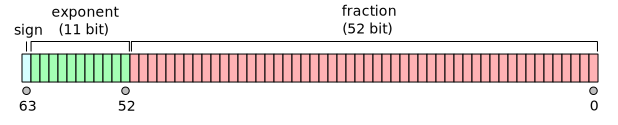
\includegraphics{img/IEEE_754.svg}
\caption{alt text}
\end{figure}

Lebegő pontos számok esetében a számítógépek egy véges számhalmazt
ábrázolnak és a számításokat is ezekkel a számokkal végzik el.
Álatalában a lebegőpontos aritmetikát használják. Ennek nézzük meg a
modelljét:

\paragraph{Definíció:}\label{definuxedciuxf3}

A nem nulla lebegőpontos számok általános alakja:

\[
\pm a^k(\frac{m_1}{a}+\frac{m_2}{a^2}+\dots+\frac{m_t}{a^t}),
\]

ahol \(a>1\) a számábrázolás alapja, \(\pm\) az előjel, \(t>1\) a
számjegyek száma és \(k\in \mathbb{Z}\) a kitevő.

Az \(m_1\) számjegy normalizált, \((1\leq m_1 \leq a-1)\) ez garantálja
a az ábrázolás egyértelműségét. A többi
számjegy:\(1\leq m_i \leq a-1 \quad (i=2,3,\dots,t)\). A nulla az nem
normalizált tehát \(k=0, m_1=m_2=\dots=m_t=0\) és az előjele általában
\(+\). A számábrázolás alpaja itt is lehet 2, 10, 16 vagy akár más is,
átalában a programozási nyelven múlik melyiket használja. Pontosság
szempontjából: - \(t=8\) egyszeres pontosság - \(t=16\) dubla pontosság

A géptől és pontosságtól függően \(m\) tárolására \(32,64\) vagy \(128\)
bit áll rendelkezésünkre (ez rendre \(4,8,16\) byte). Ezzel párhuzamosan
nő a \(k\) értékkészlete, és adott pontosság mellett:

\[
 L \leq k \leq U.
\]

A legnagyobb ábrázolható szám:

\[
M^\infty=a^U(1-a^-t)
\]

A legkissebb pedig:

\[
-M^\infty
\]

A lebegőpontos számok a \([-M^\infty,M^\infty]\)-beli számok diszkrét
(racionális) részhalmazát alkotják és ez a részhalmaz a nullára nézve
szimmetrikus. A nullához legközelebb eső lebegő pontos szám:
\(\varepsilon_0=a^{L-1}\) és az \(\varepsilon_0\)-hoz legközelebb eső
szám pedig: \(\varepsilon_0(1+a^{1-t})\).

A gép relatív pontossága vagy másképpen a gépi epszilon a
\(\varepsilon_1=a^{1-t}.\)

    \subsection{Klasszikus hiba analízis}\label{klasszikus-hiba-analuxedzis}

\paragraph{Definíció:}\label{definuxedciuxf3}

Legyen \(A\) egy pontos értékt és legyen \(a\) ennek valamilyen
közelítése. A \(\Delta a=A-a\) mennyiséget a közelítés hibájának
nevezzük és a \(|\Delta a|=|A-a|\) pedig az abszolút hibájának. Azt a
\(\delta a\) értéket pedig abszolút hibakorlátnak nevezzük amelyre
fenáll, hogy \(|A-a|=|\Delta a| \leq \delta a\).

Az \(A\) szam valamilyen közelítő értékének a relatív hibája pedig a
\(\frac {\delta a} {A}\) mennyiség

Az additív műveletek abszolút hibákorlátja pedig a következőek:

\[
\delta(a+b)\leq \delta a+ \delta b \\
\delta(a-b)\leq \delta a+ \delta b
\]

Az multiplikatív műveletek abszolút hibákorlátjai:

\[
\delta(ab) \approx |a|\delta b +|b| \delta a \\
\delta(a/b) \approx  \frac {|a|\delta b +|b| \delta a}{|b|^2}
\]

Az aritmetikai műveletek relatív hibakorlátjai a következőek, feltéve
hogy a nevező sehol sem nulla és az additív műveleteknél az operandusok
megegyező előjelűek:

\[
\frac{\delta(a+b)} {|a+b|} =  max( \frac{\delta a}{|a|}, \frac{\delta b}{|b|} ) \\
\frac{\delta(a-b)} {|a-b|} = \frac{\delta a + \delta b} {|a-b|} \\
\frac{\delta(ab)} {|ab|} \approx \frac{\delta a}{|a|} + \frac{\delta b}{|b|} \\
\frac{\delta(\frac {a}{b})} {|\frac {a}{b}|} \approx \frac{\delta a}{|a|} + \frac{\delta b}{|b|}
\]
